%\documentclass[preview, border=5mm]{standalone}
\documentclass[a3paper]{slides}

\usepackage[margin=2cm]{geometry}

% for the \xintFor***
\usepackage{xinttools} 
\usepackage{tikz}
\usetikzlibrary{calc}


% playing role of infinity (should be < .25\maxdimen)
\def\bigLen{20cm}

% define the "half plane" to be clipped (#1 = half the distance between cells)
\tikzset{
  half plane/.style={
    to path={
       ($(\tikztostart)!.5!(\tikztotarget)!#1!(\tikztotarget)!\bigLen!90:(\tikztotarget)$)
    -- ($(\tikztostart)!.5!(\tikztotarget)!#1!(\tikztotarget)!\bigLen!-90:(\tikztotarget)$)
    -- ([turn]0,2*\bigLen) -- ([turn]0,2*\bigLen) -- cycle
    }
  },
  half plane/.default={2pt},
  conector/.style={
    to path={
       (\tikztostart)
    --(\tikztotarget)
    -- cycle
    }
  },
  conector/.default={2pt}
}

% random points are in [-\maxX,\maxY]x[-\maxX,\maxY]
%\def\maxX{ 13.85 }
\def\maxX{ (\textwidth  * 0.5 }
\def\maxY{ \maxX * 1.44  }


% number of random points
\def\puntosCantidad{45} 
\def\paso{8}

\def\radio{10}
\def\centro{0}

\begin{document}

  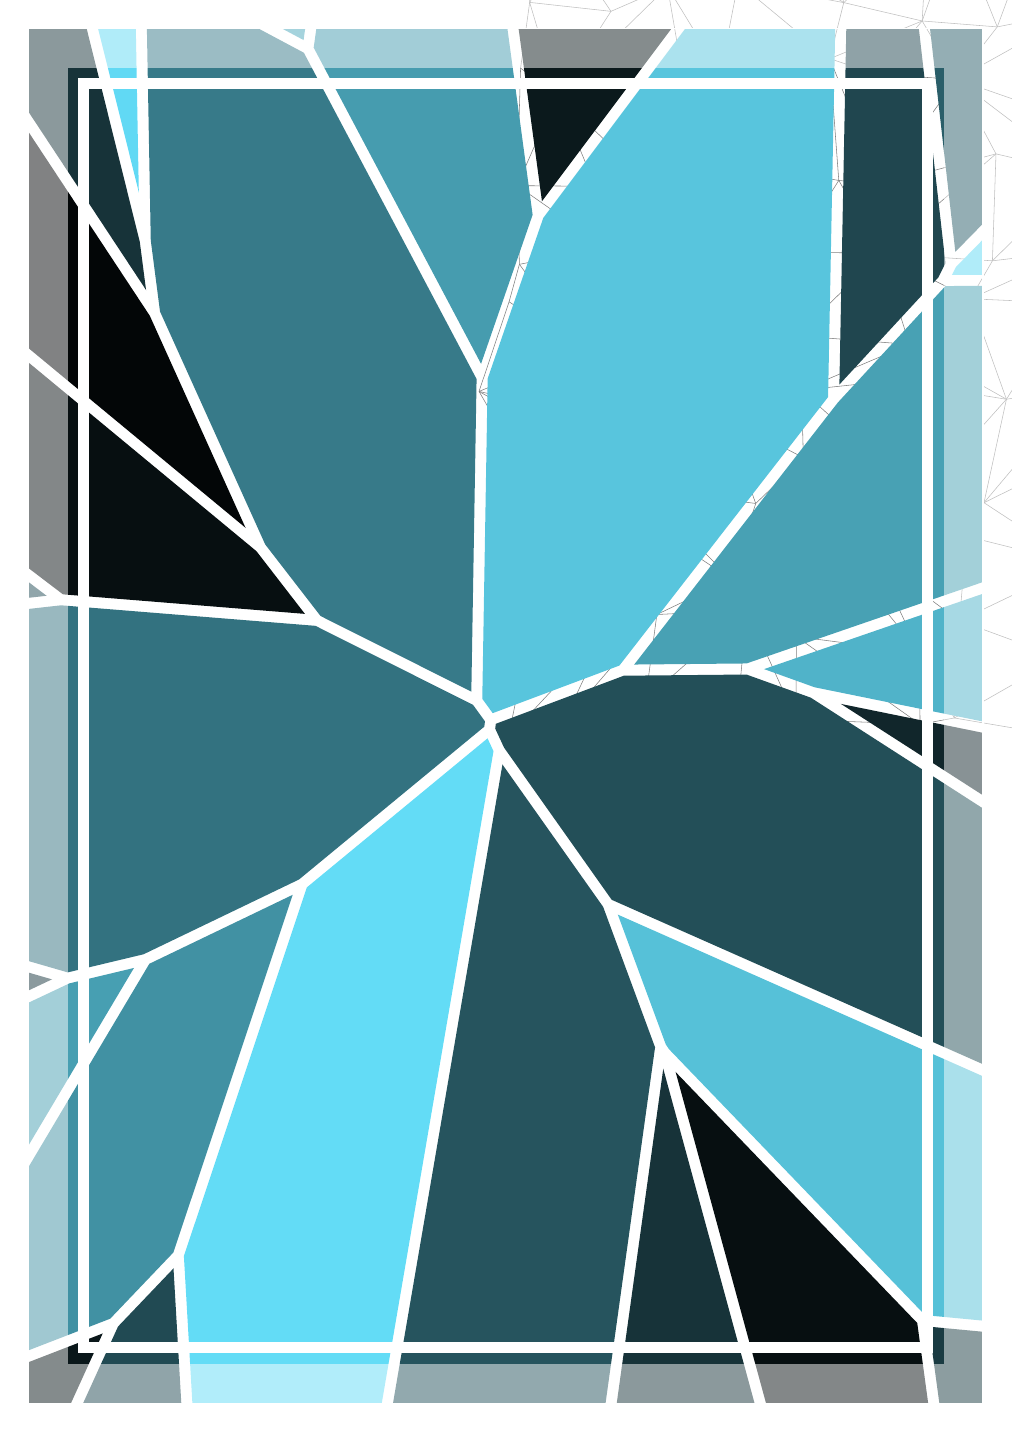
\begin{tikzpicture}
    %\draw (-\maxX,0) -- ( \maxX,0 );
    %\draw (0,-\maxY) -- ( 0,\maxY );

    % \pgfmathsetseed{1908}

    % Posicionar Puntos
    \def\cuenta{1}
    \def\puntos{}
    \xintFor* #1 in { \xintSeq {1}{\puntosCantidad} } \do{

      \def\grado{ \cuenta  }
      \edef\cuenta{\cuenta + \paso}

      \pgfmathsetmacro{\puntoX}{
        \centro 
        + ( \radio * cos( \grado ) )
        + ( rand ) 
      } 

      % random x in [-.9\maxY,.9\maxY]
      \pgfmathsetmacro{\puntoY}{ 
        \centro  
        + ( \radio * sin( \grado ) ) 
        + (rand )
      } 

      % stock the random point
      \edef\puntos{\puntos, ( \puntoX, \puntoY )} 
    }

   \foreach \i [evaluate={\ii=int(\i-1);}] in {0,...,10}{
      \foreach \j [evaluate={\jj=int(\j-1);}] in {0,...,10}{
        \coordinate [shift={(\j,\i)}] (n-\i-\j) at (rand*180:1/4+rnd/8);
%		\pgfmathsetmacro{\puntoX}{
%		        \i
%		} 
%
%		\pgfmathsetmacro{\puntoY}{ 
%		    \j
%		} 
%
%		% stock the random point
%		\edef\puntos{\puntos, ( \puntoX, \puntoY )} 
    
        \ifnum\i>0
          \draw [help lines] (n-\i-\j) -- (n-\ii-\j);
        \fi
        
        \ifnum\j>0
          \draw [help lines] (n-\i-\j) -- (n-\i-\jj);
          
    	  \ifnum\i>0
            \pgfmathparse{int(rnd>.5)}
            \ifnum\pgfmathresult=0
              \draw [help lines] (n-\i-\j) -- (n-\ii-\jj);
            \else
              \draw [help lines] (n-\ii-\j) -- (n-\i-\jj);
            \fi
          \fi
        \fi
    
      }
    }
    % draw the points and their cells
    \xintForpair #1#2 in \puntos \do{
      \edef\puntoA{#1,#2}

      \begin{scope}
        \xintForpair \#3#4 in \puntos \do{
          \edef\puntoB{#3,#4}

          % check if (#1,#2) == (#3,#4) 
          \ifx\puntoA\puntoB\relax 
            \tikzstyle{myClip}=[];
            \tikzstyle{myClip2}=[];
          \else
            \tikzstyle{myClip}=[clip ];
            \tikzstyle{myClip2}=[clip];
          \fi;
          \path [myClip] (#3,#4) to [half plane] (#1,#2);
          %\path [myClip2] (#3,#4) to [conector] (#1,#2);
          %\draw (#3,#4) -- ( #1,#2 );
        }
        % last clip
        \clip (-\maxX,-\maxY) rectangle (\maxX,\maxY); 

        \pgfmathsetmacro{\randSat}{ rnd }
        \definecolor{randcolor}{hsb}{ .53, .6, \randSat,  }
        % fill the cell with random color
        \fill[randcolor] (#1,#2) circle (14*\bigLen); 
        % and draw the point
        %\fill[draw=white,fill=white] (#1,#2) circle (4pt); 
      \end{scope}

    }

    \draw[draw=white,draw=white,line width=4pt] 
	  ({-\maxX - 20 },{-\maxY - 20 })
	  rectangle 
	  ({\maxX - 20	},{\maxY - 20 });
    \draw[draw=white,draw opacity=.5,line width=1cm] 
	  ({-\maxX },{-\maxY }) 
	  rectangle 
	  ({\maxX },{\maxY });

    \pgfresetboundingbox
	  \draw[draw=white] (-\maxX,-\maxY) rectangle (\maxX,\maxY );

  \end{tikzpicture}

\end{document}

